%--------------------------------------------------------------------------------------------------------------------
% Right lower picture: Unstructured grid
%--------------------------------------------------------------------------------------------------------------------
\begin{center}
\begin{tikzpicture}
[
 scale=0.7,
 ],
%
\node[inner sep=0pt] at (0,0)
 {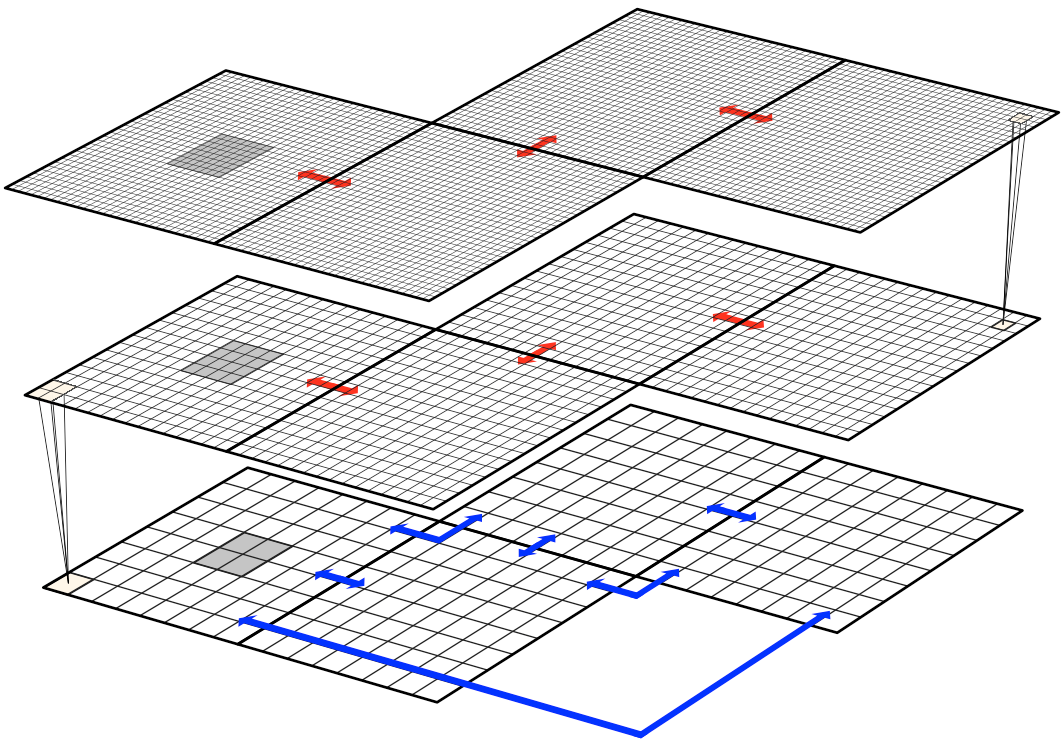
\includegraphics[width=.55\textwidth]{./\figPath/mg_method.png}};

\foreach \y in {0,1,2} {
   \pgfmathsetlengthmacro{\ypos}{(\y*2.3-3+0.7)*1cm}
   \node at (-7.8,\ypos) { \small Level \y }; 
}

%\draw [->, dashed] (0,-4) -- (0,-5) -- (8,-5) -- (8,5) -- (0,5) -- (0,4);
%\node at (4,5.5) { \small Pressure iteration }; 

\def\xposC{-15.5}
\def\yred{2.5}
\def\yblue{1.5}
\node[text=red, anchor=west] (RED) at (\xposC,\yred) { \footnotesize Local communication }; 
\draw [<->, color=red, very thick] ($ (RED.west) - (1,0) $) -- (RED.west);
\node[text=blue, anchor=west] (BLUE) at (\xposC,\yblue) { \footnotesize Global communication }; 
\draw [<->, color=blue, very thick] ($ (BLUE.west) - (1,0) $) -- (BLUE.west);

\def\xposG{-13.5}
\node[inner sep=0pt] (TRANS) at (\xposG,-1.1)
 {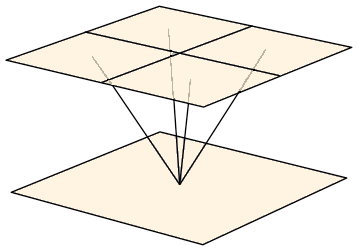
\includegraphics[scale=0.8]{./\figPath/mg_transfer.png}};
\node at ($(TRANS.south) - (0,0.5)$) { \footnotesize Grid transfer }; 

\end{tikzpicture}
\end{center}
%
